\documentclass{article}
\usepackage[slovene]{babel}
\usepackage[utf8]{inputenc}
\usepackage[T1]{fontenc}

\usepackage{amsmath}
\usepackage{amsthm}
\usepackage{amsfonts}
\usepackage{url}
\usepackage{graphicx}
\usepackage{enumerate}
\usepackage{listings}
\graphicspath{ {images/} }

\newtheorem{algoritm}{Algoritem}[section]
\newtheorem{theorem}{Izrek}[section]
\newtheorem{corollary}{Corollary}[theorem]
\newtheorem{lemma}[theorem]{Lema}
\newtheorem{trditev}{Trditev}[section]

\setlength\parindent{0pt}

\begin{document}

\begin{titlepage}
	\centering
	{\scshape\LARGE Fakulteta za matematiko in fiziko \par}
	\vspace{1cm}
	{\scshape\Large Računsko podprto geometrijsko oblikovanje\par}
	\vspace{1.5cm}
	{\huge\bfseries VS postopek za izračun vrednosti polinomov več spremenljivk\par}
	\vspace{2cm}
	{\Large\itshape Janez Radešček, Miha Avsec\par}
	\vfill

	\vfill

% Bottom of the page
	{\large \today\par}
\end{titlepage}


\section{De Casteljau}

Naj bo $T$ trikotnik v ravnini, ter naj bodo $(r,s,t)$ baricentrične koordinate točke $P$ glede na trikotnik $T$. V tem primeru lahko vsak polinom stopnje $d$, definiran nad trikotnikom $T$, zapišemo v Bernsteinovi bazi kot
$$p(r,\\s,\\t) = \sum_{i=0}^{d}\sum_{j=0}^{i}b_{d-i,i-j,j}B_{d-i,i-j,j}^{d},$$
kjer velja
$$B_{i,j,k}^{d}(r,s,t) = \frac{d!}{i!j!k!}r^{i}s^jt^k.$$

Tako podan polinom lahko evaluiramo s pomočjo De Casteljaujevega algoritma
\begin{algoritm}[De Casteljau]
Naj bo $p$ polinom stopnje $d$ podan v Bezierjevi obliki, ter naj bodo $ r,s,t$ baricentirčne koordinate točke $P$, tedaj lahko s sledečim algoritmom izračunamo vrenost polinoma p v točki $P$.
\begin{lstlisting}[escapeinside={(*}{*)}]
for k=1:d
  for i=0:d-k
      for j=0:i
           (*$b_{d-i-k,i-j,j}^k = r*b_{d-i-k+1,i-j,j}^{k-1}+s*b_{d-i-k,i-j+1,j}^{k-1} +r*b_{d-i-k,i-j,j+1}^{k-1}  $*)
(*$p(r,s,t) = b_{0,0,0}^{d}$*)
\end{lstlisting}
\end{algoritm}

\begin{trditev}
\label{decast}
De Casteljaujev algoritem potrebuje $d(d+1)(d+2)/2$ množenj.
\end{trditev}

\begin{proof}
V notranji zanki na vsakem koraku naredimo $3$ množenja. Notranja zanka se izvede $i+1$ krat. To pomeni da v drugi zanki naredimo $3(i+1)$ množenj. Vsota $\sum_{i=0}^{d-k}3(i+1) = \frac{3}{2}(d-k+1)*(d-k+2)$. Za celotno število korakov je potrebno sešteti še $\sum_{k=1}^{d}\frac{3}{2}(d-k+1)*(d-k+2) = d(d+1)(d+2)/2$.
\end{proof}



\section{Modificirana Bernstein-Bezierjeva reprezentacija}

Če imamo podan polinom v Bernsteinovi obliki $$p(r,\\s,\\t) = \sum_{i=0}^{d}\sum_{j=0}^{i}b_{d-i,i-j,j}B_{d-i,i-j,j}^d(r,\\s,\\t),$$
potem lahko tak polinom enostavno prepišemo v obliko
$$p(r,\\s,\\t) = \sum_{i=0}^{d}\sum_{j=0}^{i}c_{d-i,i-j,j}r^{d-i}s^{i-j}t^j,$$
tako da za koeficiente $c_{d-i,i-j,j}$ vzamemo
$$c_{d-i,i-j,j} = \frac{d!}{(d-i)!(i-j)!j!}b_{d-i,i-j,j}, \quad j=0,\ldots, i;\\ i = 0,\ldots,d.$$
Tej obliki polinoma rečemo modificirana Bernstein-Bezierjeva oblika ali krajše MBB. Pokazati želimo, da se polinom v MBB obliki, da evaluirati hitreje kakor v klasični Bezierjevi obliki. Ideja, ki se skriva v ozadju je ta, da lahko $p$ zapišemo v gnezdeni obliki. Poglejmo si na primeru polinomov stopnje $2$. Označimo kontrolne točke na sledeči način:

\begin{center}
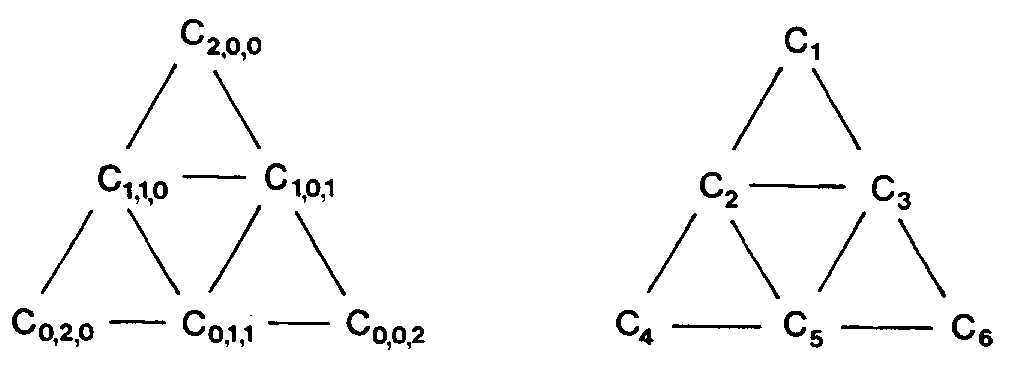
\includegraphics[width=.9\linewidth]{graf.png}
\end{center}

Če razpišemo sedaj polinom glede na spremenljivko $r$ dobimo:

\begin{align}
p(r,s,t) &= \sum_{i=0}^{2}\sum_{j=0}^{i}c_{2-i,i-j,j}r^{2-i}s^{i-j}t^j \nonumber \\ \nonumber
&= r^2\sum_{j=0}^{0}c_{2,-j,j}s^{-j}t^j + r\sum_{j=0}^{1}c_{1,1-j,j}s^{1-j}t^j + \sum_{j=0}^{2}c_{0,2-j,j}s^{2-j}t^j \\ \nonumber
&= r^2(c_1) + r(c_2s+c_3t) + (c_4s^2+c_5st+c_6t^2)\\ \nonumber
&= r^2(c_1+\frac{s}{r}c_2+\frac{t}{r}c_3+\frac{s^2}{r^2}c_4+\frac{st}{r^2}c_5+\frac{t^2}{r^2}c_6) \\ \nonumber
&= r^2(\frac{s}{r}(c_2+\frac{s}{r}c_4+\frac{t}{r}c_5)+\frac{t}{r}(\frac{t}{r}c_6+c_3)+c_1) \nonumber
\end{align}

Tu je potrebno biti pozoren na to, da ne delimo z $0$. Temu se lahko izognemo tako, da ločimo primere glede na to kje v kontrolnem trikotniku se nahajamo. Ločimo $3$ primere kot je prikazano na sliki.

\begin{center}
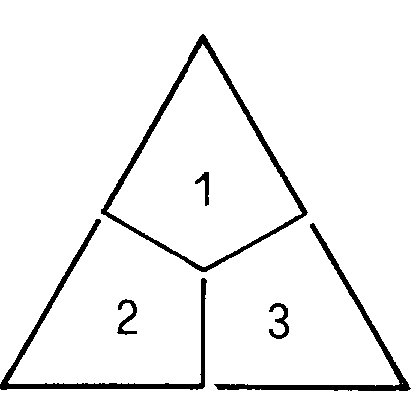
\includegraphics[width=.3\linewidth]{graf1.png}
\end{center}
Posamezne regije so določena na sledeč način
\begin{enumerate}
\item  $r \geq s, r \geq t$
\item $s > r, s \geq t$
\item $t>r, t>s$
\end{enumerate}

S pravilno izbiro regije poskrbimo, da ne delimo z $0$, hkrati pa se izognemo še deljenju z zelo majhnimi števili, ki bi jih dobili pri baricentričnih koordinatah blizu roba.

Zgornji primer lahko posplošimo na polinome poljubnih dimenzij.

\begin{algoritm}
\label{MBB}
Naj bo p polinom stopnje $n$ podan v MBB obliki, ter naj bodo $ r,s,t$ baricentirčne koordinate točke za katere velja $r \geq s,r \geq t$, tedaj lahko s sledečim algoritmom izračunamo vrenost polinoma p v točki $(r,s,t)$
\begin{lstlisting}[escapeinside={(*}{*)}]
sr = s/r,	 tr= s/r
A = (*$c_{0,n,0}$*);
for i = 1:n
    B = (*$c_{0,n-i,i}$*)
    for j = i:-1:1
        B = B*tr + (*$c_{i-j+1,n-i,j-1}$*);
    end
    A = A *sr +B;
end
p(r,s,t) = A(*$r^n$*)
\end{lstlisting}
\end{algoritm}

\begin{trditev}
Algoritem za izračun vrednosti polinoma v MBB obliki potrebuje $(n^2+5n)/2$ množenj.
\end{trditev}
\begin{proof}
Sledimo postopku iz dokaza trditve \ref{decast}.
\end{proof}
Tu je potrebno povedati, da se lahko $r^n$ izračuna hitreje, kot z $n-1$ množenji, torej je samo število operacij v algoritmu še nekoliko manjše. Podobno lahko izpeljemo tudi algoritme za ostala območja.


\vspace{3mm}

Pojavlja se še vprašanje zahtevnosti pretvorbe polinoma v MBB obliko. Če se lotimo naivno in na novo poračunamo vse koeficiente potem nas ta postopek stane $O(n^3)$ operacij. Kar lahko povzroči to, da je časovna zahtevnost, ki jo potrebujemo za izračun ene točke večja, kot če bi uporabili navadni De Casteljaujev algoritem. Še vedno pa bo veljalo, da v primeru če želimo izračunati veliko točk na istem polinomu MBB algoritem deluje veliko hitreje.

Druga možnost, ki jo imamo pa je ta, da si v naprej poračunamo vrednosti s katerimi moramo množiti koeficiente polinoma. To je potrebno za vsako dimenzijo storiti le enkrat, nato pa za izračun novih koeficientov potrebujemo le še $(d^2+3d-4)/2$ množenj. Temu postopku rečemo VSC algoritem. VSC algoritem je tako vedno bolj učinkovit kot De Casteljaujev algoritem.

\newpage

\section{Polinom v Taylorjevi vrsti}

Naj bo T trikotnik in naj bo $p$ polinom stopnje $n$ definiran na $T$. Naj bosta $u = x-x_1$ in $v = y-y_1$ določena na tak način. Tu sta $(x_1,y_1)$ koordinati poljubnega ogljišča trikotnika. Polinom $p$ lahko potem zapišemo v Taylorjevi obliki kot 
$$p(u,v) = \sum_{i = 0}^n{\sum_{j=0}^{n-i}{a_{i,j}u^iv^j }}.$$To obliko bomo krajše klicali $TAY$.  Vrednost polinoma $p$ v točki $(u,v)$ lahko izračunamo s sledečim algoritmom.

\begin{algoritm}
\begin{lstlisting}[escapeinside={(*}{*)}]

p = (*$a_{0,n}$*)
for i = 1:d
    A = (*$a_{i,n-i}$*)
    for j = 1:i
        A = A * u + (*$a_{i-j,n-i}$*)
    end
    p = p * v + A
end
\end{lstlisting}
\end{algoritm}

\begin{trditev}
Taylorjev algoritem za izračun vrednosti polinoma potrebuje $(n^2+3n)/2$ množenj.
\end{trditev}

\begin{proof}
Sledimo postopku iz dokaza trditve \ref{decast}.
\end{proof}

\section{Primerjava algoritmov}

Algoritmu \ref{MBB}, ki ne potrebuje pretvorbe iz Bernsteinove v MBB obliko nakratko rečemu VS algoritem. V spodnji tabeli lahko vidimo primerjavo števla množenj, ki jih posamezen algoritem izvede odvisno od stopnje polinoma.

\begin{center}
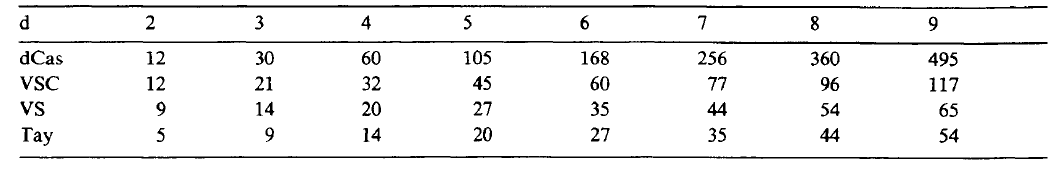
\includegraphics[width=.9\linewidth]{tabelca.PNG}
\end{center}

 Če povzamemo imamo na tem mestu sledeče časovne zahtevnosti, pri kateri smo poleg množenj dodali še deljenja, ki pa ne vplivajo bistevno na število operacij, ki jih moramo izvesti.

\begin{align}
(d^3+3d^2+2d)/2& \quad \text{de Casteljou} \nonumber \\
(2d^2+8d)/2& \quad \text{VSC} \nonumber \\
(d^2+5d+4)/2& \quad \text{VS} \nonumber \\
(d^2+3d)/2& \quad \text{Taylor} \nonumber
\end{align}

Tu je jasno vidno, da ima edino de Casteljoujev algoritem kubično zahtevnost, ostali algoritmi pa le kvadratično. Velikost razlike v številu množenj lahko jasno vidimo v zgornji tabeli. Opazimo tudi, da je Taylorjev algoritem najhitrejši. Vendar nas sama pretvorba iz Bernsteinove ali MBB oblike v Taylorjevo stane preveč, da bi se nam splačalo izvajati Taylorjev algoritem. Zaključimo lahko torej, da je v primeru, ko delamo z polinomi v Bernsteinovi obliki najboljši VSC algoritem.


\section{Polinomi na tetraedrih}

Naj bo T tetraeder. Za vsako točko $U$ iz $T$ naj bodo $(r,s,t,u)$ pripadajoče Baricentrične koordinate glede na $T$.  Naj bo $p$ polinom stopnje $n$ definiran na $T$. Polinom $p$ lahko zapišemo v modificirani Bernstein-Bezierjevi obliki kot 
$$p(r,s,t,u) = \sum_{i = 0}^n{\sum_{j=0}^{i}{\sum_{k = 0}^{j}{c_{d-i,i-j,j-k,k} r^{d-i} s^{i-j} t^{j-k} u^k}}}.$$
Tako podan polinom ima $(d+1)(d+2)(d+3)/6$ koeficientov. Na sliki lahko vidimo te koeficiente v primeru $d=2$.

\begin{center}
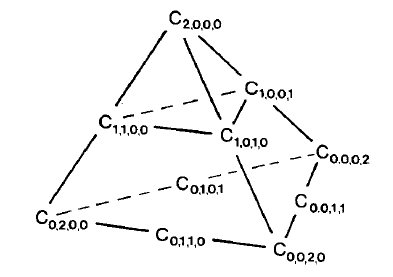
\includegraphics[width=.7\linewidth]{tetraeder.PNG}
\end{center}

Kot v dvodimenzionalnem primeru, uporabimo nekoliko drugačen algoritem glede na to kje točka $(r, s, t, u)$ leži v tetraedru.
Definiramo štiri regije tetraedra.

\begin{enumerate}
\item $r\geq s, r\geq t, r\geq u$
\item $s\geq r, s\geq t, s\geq u$
\item $t\geq r, t\geq s, t\geq u$
\item $u\geq r,u\geq s, u\geq t$
\end{enumerate}

%zavrtimo točke tako da je računanje efficient

Vrednost polinoma $p$ v točki $(r,s,t,u)$, ki se nahaja v četrti regiji, lahko izračunamo s sledečim algoritmom.

\begin{algoritm}
Naj bo p polinom stopnje $d$ podan v MBB obliki, ter naj bodo $ r,s,t,u$ baricentirčne koordinate točke za katere velja $u > r,u > s, u>t$, tedaj lahko s sledečim algoritmom izračunamo vrenost polinoma p v točki $(r,s,t,u)$

\begin{lstlisting}[escapeinside={(*}{*)}]
ru = r/u,	 su= s/u	 tu= t/u
A = (*$c_{n,0,0,0}$*);
for i = 1:n
    B = (*$c_{n-i,i,0,0}$*)
    for j = 1:i
        C =  (*$c_{n-i,i-j,j,0}$*)
            for k = 1:j
                C = C * tu + (*$c_{n-i,i-j,j-k,k}$*)
            end
        B = B * ru + C
    end
    A = A * ru + B;
end
p(r,s,t,u) = A(*$u^n$*)
\end{lstlisting}
\end{algoritm}

\begin{trditev}
Zgornji algoritem za izračun vrednosti polinoma potrebuje $(d^3+ 6d^2 + 17d)/6$ množenj.
\end{trditev}

\begin{proof}
Sledimo postopku iz dokaza trditve \ref{decast}.
\end{proof}

Na podoben način lahko izepeljemo tudi algoritme za polinome več spremenljivk.


\begin{thebibliography}{9}

\bibitem{referenca-clanek}
Larry~L.~Schumaker, Wolfgang ~Volk, \emph{Efficient evaluation of multivariate
polynomials}, Computer Aided Geometric Design 3, North-Holland (1986) 149--154.

\end{thebibliography}

\end{document}